% TU Delft beamer template
% Author: Erwin Walraven (initial version was created by Maarten Abbink)
% Delft Universiy of Technology

\documentclass[xcolor=dvipsnames,aspectratio=169]{beamer}
\usepackage[english]{babel}
\usepackage{graphicx}
\usepackage{subfig}
\usepackage{amsmath}
\usepackage{amsfonts}
\usepackage{amsthm}

\usepackage{tikz}
\usepackage{pgfplots}
\usetikzlibrary{positioning,backgrounds,fit}
\usetikzlibrary{arrows, arrows.meta, calc, quotes, shapes}
\usetikzlibrary{intersections, pgfplots.fillbetween}
\usetikzlibrary{decorations.pathreplacing}


\usetikzlibrary{pgfplots.groupplots}
\usetikzlibrary{patterns}

\definecolor{pblue}{rgb}{0.12156863,  0.46666667,  0.70588235}
\definecolor{porange}{rgb}{1.        ,  0.49803922,  0.054901965}
\definecolor{pgreen}{rgb}{0.17254902,  0.62745098,  0.17254902}
\definecolor{pgrey}{rgb}{0.5,0.5,0.5}

\setbeamertemplate{navigation symbols}{} % remove navigation symbols
\mode<presentation>{\usetheme{tud}}

% BIB SETTINGS
\usepackage[backend=bibtex,firstinits=true,maxnames=30,maxcitenames=20,url=false,style=authoryear]{biblatex}
\bibliography{bibfile}
\setlength\bibitemsep{0.3cm} % space between entries in the reference list
\renewcommand{\bibfont}{\normalfont\scriptsize}
\setbeamerfont{footnote}{size=\tiny}
\renewcommand{\cite}[1]{\footnote<.->[frame]{\fullcite{#1}}}


\title[]{Data-Driven and Modular Control \\ for Controlled Environment 
Agriculture}
\institute[]{Delft University of Technology, The Netherlands}
\author{Robert D. (Koty) McAllister}
%\date{}

\begin{document}
{
\setbeamertemplate{footline}{\usebeamertemplate*{minimal footline}}
\frame{\titlepage}
}

{\setbeamertemplate{footline}{\usebeamertemplate*{minimal footline}}

}

\begin{frame}{My background: Plants}

\centering
\begin{tikzpicture}[font=\normalsize]
	
	\only<2->{
	\node[align=center,name=atext] at (0,0) {Chemical \\ reactions \medskip \\ 
	Vapor-liquid \\ equilibrium};
	\node[align=center,name=apic] at (2.8,0) 
	{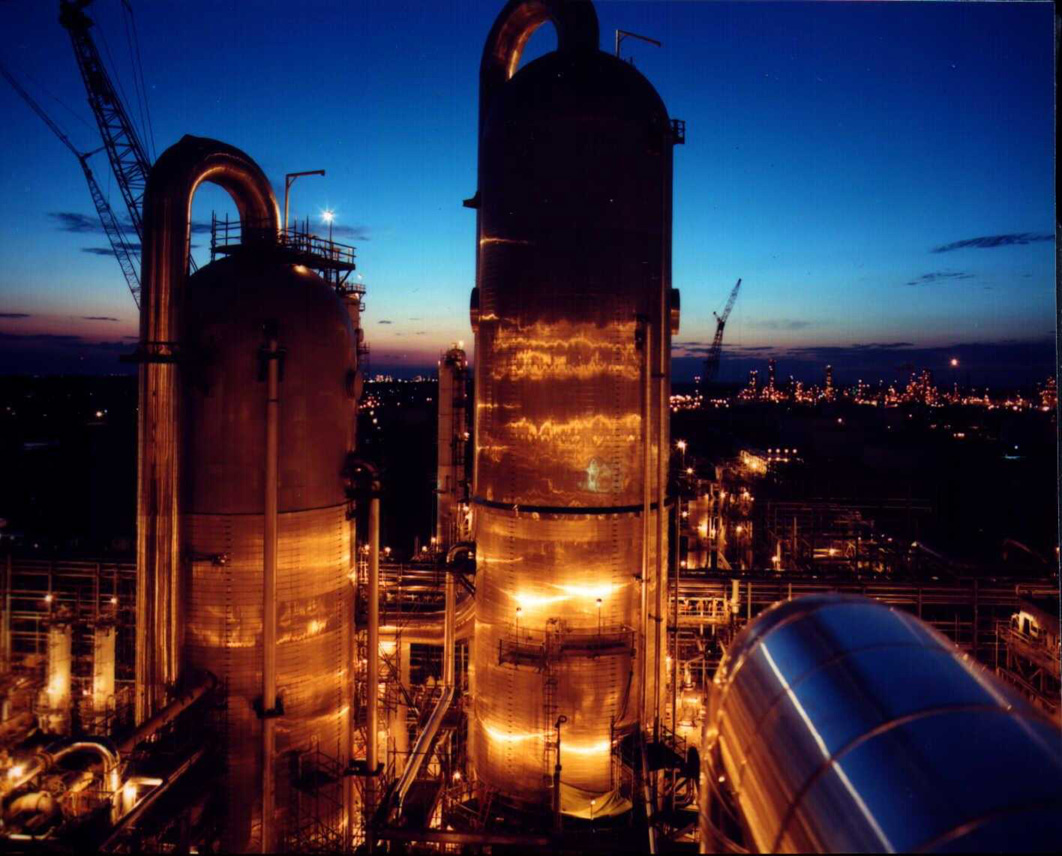
\includegraphics[width=0.21\linewidth]{BasfNightshot.jpg}};
	\node[align=center,name=middle] at (5.9,0) {Economic \\ optimization 
	\medskip \\ Heat \& mass \\ transport};
	\scoped[on background layer]{\node [fit=(atext)(apic)(middle), rounded 
	corners=10mm,draw=porange,fill=porange!30,opacity=0.5,line width= 2pt] {};}
	}
	\only<3->{
		\node[align=center,name=bpic] at (9,0) 
		{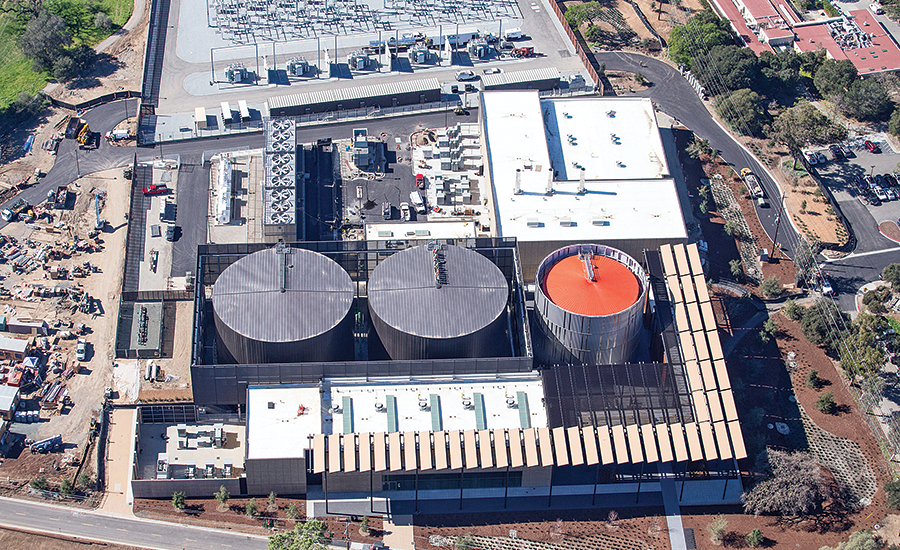
\includegraphics[width=0.21\linewidth]{Johnson_controls_ENRready.png}};
		\node[align=center,name=bpic,opacity=0] at (9,0) {
			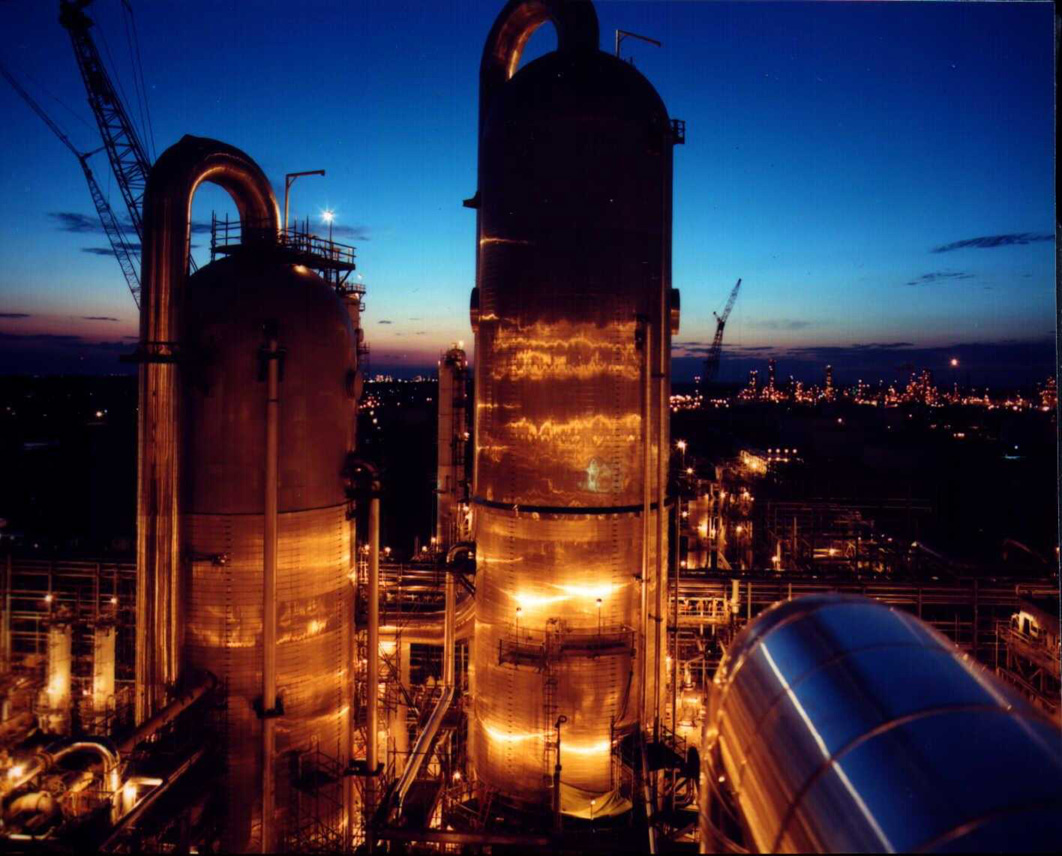
\includegraphics[width=0.21\linewidth]{BasfNightshot.jpg}};
		\node[align=center,name=btext] at (11.8,0) {Time-varying \\ systems 
		\medskip \\ Weather-based \\ disturbances};
		\scoped[on background layer]{\node [fit=(btext)(bpic)(middle), rounded 
		corners=10mm,draw=pblue,fill=pblue!30,opacity=0.5,line width= 2pt] {};}
	}
	
	\scoped[on background layer]{\draw [ rounded 
	corners=10mm,draw=pgreen,fill=pgreen!30,opacity=0,line width= 2pt] 
	(-1.4,-4.5) rectangle (13.3,1.8);}
	\only<4->{
		\node[align=center,name=c] at (5.9,-3) 
		{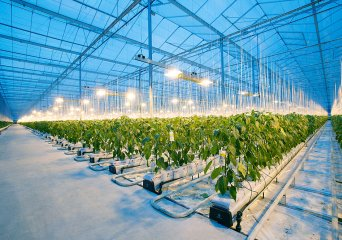
\includegraphics[width=0.25\linewidth]{greenhouse.jpg}};
		\node[align=center] at (1.9,-3) {Biological \\ systems};
		\node[align=center] at (9.9,-3) {Time-scale \\ separation};
		\scoped[on background layer]{\draw [ rounded 
		corners=10mm,draw=pgreen,fill=pgreen!30,opacity=0.5,line width= 2pt] 
		(-1.4,-4.5) rectangle (13.3,1.8);}
	}
\end{tikzpicture}

\end{frame}

\begin{frame}{Controlled environment agriculture (CEA)}
	
	\vspace{0.5cm}
	
	\centering
	\begin{tikzpicture}
	\node[align=center] at (0.5,5) {Heat/cool \\ Light \\ Dehumidify \\ 
	CO\textsubscript{2} Injection};
	\draw[->,>=stealth,line width=2pt] (2,5) -- (3,5);
	\node at (5,5) {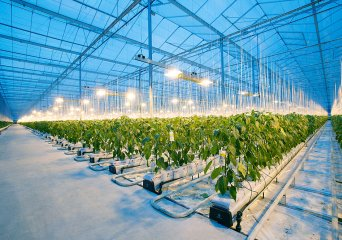
\includegraphics[width=0.25\linewidth]{greenhouse.jpg}};
	\draw[->,>=stealth,line width=2pt] (7,5) -- (8,5);
	\node[align=center] at (9.5,5) {T, RH\%, CO\textsubscript{2} \\ Biomass};

	\draw[->,>=stealth,line width=2pt] (2,8) -| (5,6.5);
	\node[align=center] {};
	
	\draw [very thick, decorate,decoration={brace,amplitude=8pt}] (1.7,4) -- 
	(-0.7,4) node[align=center,pos=0.5,below=10pt] {\Large $u$};
	\draw [very thick, decorate,decoration={brace,amplitude=8pt}] (10.7,4) -- 
	(8.3,4) node[align=center,pos=0.5,below=10pt] {\Large $x$};
	\draw [very thick, decorate,decoration={brace,amplitude=8pt}] (-1.2,7) -- 
	(-1.2,9) node[align=center,pos=0.5,left=10pt] {\Large $d$};
	\begin{scope}
		[
		ax/.style={thick, draw=black, cap=rect,line width=1pt},
		xshift=-1cm,
		yshift=7cm,
		yscale=0.5,
		xscale=0.5,
		]
		
		\draw[ax,->,>=stealth] (0, 0.2) -- (4.8, 0.2) node[right] {$t$};
		\draw[ax,->,>=stealth] (0, 0.2) -- (0, 4);
		
		\draw [color=pblue,line width=1pt] plot [domain=0:4.3,smooth] 
		(\x,{3.4-0.4*sin(1.5*\x r)});
		\node[color=pblue,right] at (4.3,3.45) {T\textsubscript{a}};
		
		\draw [color=porange,line width=1pt] plot [smooth] 
		coordinates 
		{(1,2) (1.5,2.5) (2,2.6) (2.5,2.8) (3,2.6) (3.5,2)};
		\draw [color=porange,line width=1pt] plot
		coordinates {(0,2) (1,2)};
		\draw [color=porange,line width=1pt] plot
		coordinates {(3.5,2) (4.3,2)};
		\node[color=porange,right] at (4.3,2) {I\textsubscript{a}};
		
		\draw [color=pgreen,line width=1pt] plot [smooth] 
		coordinates 
		{(0,1) (0.5,0.9) (1,1.1) (1.5,1.3) (2,1.4) (2.5,1.4) (3,1.6) (3.5,1.4) 
		(4,1.1) (4.3,1)};
		\node[color=pgreen,right] at (4.3,1) {RH\textsubscript{a}};
		%		\node[color=porange,right] at (8,1.8) {$\textrm{Pr}(T_a(t))$};
	\end{scope}
	%			\node[align=center] at (6.5,-2.5) {$\begin{aligned}
			%					\min \ & \sum_{k=0}^{N-1}\ell(x(k),u(k),k) \\  
			%					\textrm{s.t. } & x(k+1) = f(x(k),u(k),k) \\
			%					& (x(k),u(k))\in\mathbb{Z}(k)
			%			\end{aligned}$};
	
	\end{tikzpicture}
\end{frame}

\newcommand{\greenhouse}[3]{
\draw[line width=1pt] ($ #1 + (0,0) $) rectangle ($ #1 + (#2,#3)$);
\draw[line width=1pt] ($ #1 + (0,#3) $) -- ($ #1 + (0.5*#2,1.25*#3) $);
\draw[line width=1pt] ($ #1 + (#2,#3) $) -- ($ #1 + (0.5*#2,1.25*#3) $);
}

\begin{frame}{Why is the CEA problem so difficult?}
	\centering
	\begin{tikzpicture}[circle dotted/.style={dash pattern=on .05mm off 6mm,
			line cap=round}]
		\greenhouse{(0,0)}{2}{2}
		\draw[->,>=stealth,line width = 2pt] (1,-1) -- (1,0.5);
		\node at (1,-2) {
\includegraphics[width=2cm]{lettuce.png}};
		\onslide<2->{
		\greenhouse{(2.5,0)}{2}{1.2}
		\greenhouse{(5,0)}{1.5}{1.5}
		\draw[->,>=stealth,line width = 2pt] (1,-1) -- (3.5,0.5);
		\draw[->,>=stealth,line width = 2pt] (1,-1) -- (5.75,0.5);
		\draw[line width = 2mm,circle dotted] (7.5,1) -- (9,1);
		}
		
		\onslide<3->{
		\node at (3.5,-2) {
\includegraphics[width=2cm]{tomato.png}};
		\node at (6,-2) {
\includegraphics[width=1.5cm]{cucumber.png}};
		
		\draw[line width = 2mm,circle dotted] (7.5,-2) -- (9,-2);
		}
	\end{tikzpicture}
	\onslide<4->{
	\begin{block}{}
		\centering
		Many systems with similar physics, but significantly different 
		parameters.
	\end{block} 
	}
\end{frame}

\begin{frame}{A solution: Data-driven and modular controller design}
	
	\vspace{0.3cm} 
	
	\centering
	\begin{tikzpicture}[font=\footnotesize]

		\draw[line width=2pt,name=sys] (0,0) rectangle (1.5,1) 
		node[align=center, pos=.5] {System};
		\draw[line width=2pt,name=data] (2.25,0) rectangle (3.75,1) 
		node[align=center,pos=.5] {Data}; 
		\draw[line width=2pt, ->,>=stealth,color=red] (1.5,2) 
		node[left,align=center] 
		{\textbf{Engineering} \\ \textbf{judgment}} -| (3,1);
		\draw[line width=2pt, ->,>=stealth] (1.5,0.5) -- (2.25,0.5);
		\draw[line width=2pt, ->,>=stealth] (8.25,0.5) -- (9,0.5) 
		node[right] {Deploy!};
		
		\only<1>{
		\draw[line width=2pt, ->,>=stealth] (3.75,0.5) -- (4.5,0.5);
		\draw[line width=2pt, ->,>=stealth] (6,0.5) -- (6.75,0.5);
		\node[align=center,font=\large] at (-2,1) {Model-based \\ controller 
			design};
		\draw[line width=2pt] (4.5,0) rectangle (6,1) 
		node[align=center,pos=.5] {Model}; 
		\draw[line width=2pt] (6.75,0) rectangle (8.25,1) 
		node[align=center,pos=.5] {Controller \\ design};
		\draw[line width=2pt, ->,>=stealth,color=red] (2,2) -| (5.25,1);
		\draw[line width=2pt, ->,>=stealth,color=red] (2,2) -| (7.5,1);
		}
		
		\only<2->{
		\node[align=center,font=\large] at (-2,1) {\emph{Model-free} \\ 
				controller design};
		\draw[line width=2pt] (4.5, 0) rectangle (8.25, 1) 
		node[align=center,pos=0.5] {\emph{Model-free} controller 
		\\ design (RL, DD-MPC)};
		\draw[line width=2pt, ->,>=stealth] (3.75,0.5) -- (4.5,0.5);
		\draw[line width=2pt, ->,>=stealth,color=red] (2,2) -| (6.325,1);
		}
		
		\draw[dashed] (-0.5,-0.5) -- (11,-0.5);
		
		\begin{scope}[yshift=-3.2cm]
			\only<3->{
				\node[align=center,font=\large] at (-2,1) {Modular \\ 
				controller design};
				\draw[line width=2pt, ->,>=stealth] (1.5,0.5) 
				node[left,align=center] {Application} -- (2.25,0.5);
				\draw[line width=2pt, ->,>=stealth,color=red] (1.5,2) 
				node[left,align=center] {\textbf{Engineering} \\ 
				\textbf{judgment}} -| (3.75,1);
				\draw[line width=2pt,name=sys] (2.25,0) rectangle (5.25,1) 
				node[align=center, pos=.5] {Controller synthesis \\ procedure 
				(CSP)};
				
				\draw[line width=2pt] (6.5,1.25) rectangle (7.75,2) 
				node[align=center, pos=.5] {Sys. 1};
				\draw[line width=2pt, ->,>=stealth] (7.75,1.625) -- (8.5,1.625);
				\draw[line width=2pt] (8.5,1.25) rectangle (9.75,2) 
				node[align=center, pos=.5] {CSP};
				\draw[line width=2pt, ->,>=stealth] (9.75,1.625) -- 
				(10.5,1.625) 
				node[right] {Deploy!};
				
				\node[align=center] at (7.125,1) {\Large $\vdots$};
				\node[align=center] at (9.125,1) {\Large $\vdots$};
				\node[align=center] at (11.15,1) {\Large $\vdots$};
				
				\draw[line width=2pt] (6.5,-0.25) rectangle (7.75,0.5) 
				node[align=center, pos=.5] {Sys. N};
				\draw[line width=2pt, ->,>=stealth] (7.75,0.125) -- (8.5,0.125);
				\draw[line width=2pt] (8.5,-0.25) rectangle (9.75,0.5) 
				node[align=center, pos=.5] {CSP};
				\draw[line width=2pt, ->,>=stealth] (9.75,0.125) -- 
				(10.5,0.125) 
				node[right] {Deploy!};
			}
			\draw[dashed,opacity=0] (-0.5,-0.3) -- (12,-0.3);
		\end{scope}
	\end{tikzpicture}
	
\end{frame}

\begin{frame}{Applications to CEA}
	Figures to show idea of mix-match models
\end{frame}

\begin{frame}{A natural hierarchy}
	(1) What conditions maximization plant growth with minimum energy cost? 
	(Grower) (2) 
	How do we realize these conditions (rule-based/heuristic control)? 
\end{frame}

\begin{frame}{A tool for every job}
	
\end{frame}





\end{document}
